\subsection{Der neuronale Multiplikator}
Mit der Einführung der Burgersgleichung wird nun ersichtlich, dass das neuronale Netzwerk unter anderem eine Multiplikation 'erlernen' muss. Die Multiplikation zweier Zahlen ($a \cdot b$) ist für uns einfach, jedoch ist dies für ein neuronales Netzwerk deutlich anspruchsvoller. Ein KNN mit einem hidden layer erlernt eine Summe von Funktionen analog der Gleichung \ref{mst:sum_knn}.

% CHECK IF BIAS IS CORRECT!
\begin{equation}
O = \sigma_{2} \left(\sum_{i}^{n}{\sigma_{1} (\omega_{i} \cdot I_{i} + b_i)} \right)
\label{eq:mst_sum_knn}
\end{equation}

Es gilt nun zu zeigen, dass mit Hilfe einer Summe von Aktivierungsfunktionen ($\sigma$) es möglich ist eine gute Näherung zur einfachen Multiplikation zu finden. Durch den Satz von Stone-Weierstrass ist bewiesen, dass jede stetige Funktion durch einfachere Funktionen bliebig gut auf einem Interval $[a, b]$ approximiert werden kann. Aus diesem Satz kann angenommen werden, das auf dem Interval $[a,b]$ die Multiplikation beliebig gut gelernt werden kann. Mit steigender Anzahl Neuronen sinkt somit der Fehler. Um diese Hypothese zu bestätigen, wurde ein Netzwerk verwendet, welches gemäss der Abbildung \ref{fig:mst_variable_hidden_layer} implementiert wurde. Die Neuronen im hidden Layer sind variabel zwischen 2 und 14 gewählt und das Interval umfasst $[0, 10)$. Die Daten wurden mitthilfe von 2 zufällig initialisierten Arrays erstellt. Die Zahlen sind diskretisiert in $0.1$ Schritten. Es existieren somit theoretisch 10000 kombinationen, 5000 Datenpunkte wurden verwedet um die Netzte zu trainieren.

\begin{figure}[h]
	\centering
	\begin{tikzpicture}
	\node[inputNode, thick] (i1) at (6, 0.5) {};
	\node[inputNode, thick] (i2) at (6, -0.5) {};
	
	\node[inputNode, thick] (h1) at (8, 1.5) {};
	\node[inputNode, thick] (h2) at (8, 0.75) {};
	\node[inputNode, thick] (h3) at (8, 0) {};
	
	\node[inputNode, thick] (h5) at (8, -1.5) {};
	
	\node[inputNode, thick] (o1) at (10, 0.0) {};
	
	
	\draw[stateTransition] (5, 0.5) -- node[above] {$I_1$} (i1);
	\draw[stateTransition] (5, -0.5) -- node[above] {$I_2$} (i2);
	
	
	\draw[stateTransition] (i1) -- (h1);
	\draw[stateTransition] (i1) -- (h2);
	\draw[stateTransition] (i1) -- (h3);
	\draw[stateTransition] (i1) -- (h5);
	\draw[stateTransition] (i2) -- (h1);
	\draw[stateTransition] (i2) -- (h2);
	\draw[stateTransition] (i2) -- (h3);
	\draw[stateTransition] (i2) -- (h5);
	
	\draw[stateTransition] (h1) -- (o1);
	\draw[stateTransition] (h2) -- (o1);
	\draw[stateTransition] (h3) -- (o1);
	\draw[stateTransition] (h5) -- (o1);
	
	\node[above=of i1, align=center] (l1) {Input \\ layer};
	\node[right=2.3em of l1, align=center] (l2) {Hidden \\ layer};
	\node[right=2.3em of l2, align=center] (l3) {Output \\ layer};
	
	\node[above=1.15em of h5, align=center] (l4) {...};
	
	\draw[stateTransition] (o1) -- node[above] {$O_1$} (11, 0);
	\end{tikzpicture}
	\label{fig:mst_variable_hidden_layer}
	\caption{Topologie des neuronalen Netzwerks mit variablem hidden Layer zum Trainieren der Multiplikationsoperation.}
\end{figure}

Wie aus den Resultaten in Abbildung \ref{fig:mst_multiplicator_error} unschwer zu erkennen ist, sinkt der relative Fehler mit zunehmender Neuronen Anzahl. Weiter ist unschwer zu erkennen, dass ausserhalb des Intervals $[0, 10)$ der Fehler stark zu nimmt. (A.M. fragen: Runge Phänomen? Warum weniger oszilation bei N=14 als bei N=2, weil gem. Runge würde anhand der Stüzstellen schlechtere Generalisierung als wenn N grösser ist erwarten...?)
\begin{figure}
	\centering
	\begin{tabular}{cc}
		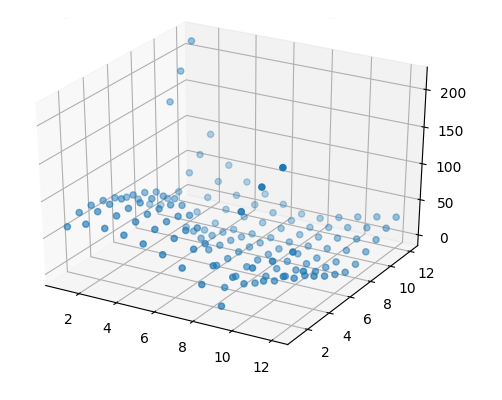
\includegraphics[scale=0.4]{learning/img/abs_plot_2_clean.png} &
		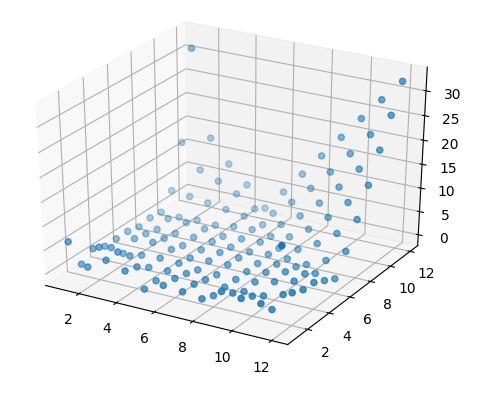
\includegraphics[scale=0.4]{learning/img/abs_plot_6_clean.png} \\
		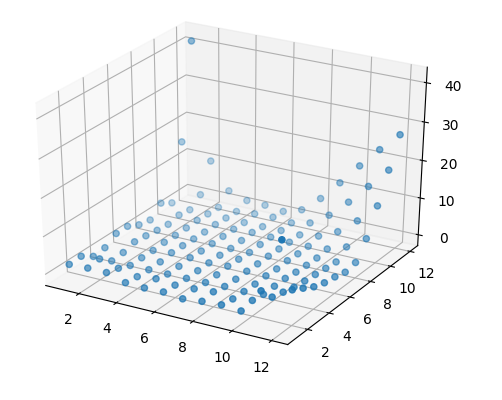
\includegraphics[scale=0.4]{learning/img/abs_plot_10_clean.png} &
		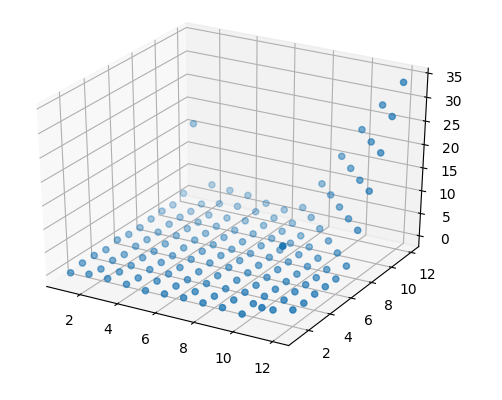
\includegraphics[scale=0.4]{learning/img/abs_plot_14_clean.png} \\				
	\end{tabular}
	\label{fig:mst_multiplicator_error}
	\caption{4 trainierte Neuronale Netzwerke mit 2 (\textit{oben links}), 6, 10 und 14 ( \textit{unten rechts}) Nodes im hidden Layer. Die blauen Punkte stellen sämtliche Kombinationen in X, Y auf dem Interval $[0,12)$ dar um zu verdeutlichen, wie sich der Fehler ausserhalb des trainierten Intervals $[0,10)$ entwickelt.}
\end{figure}

\begin{figure}
	\centering
	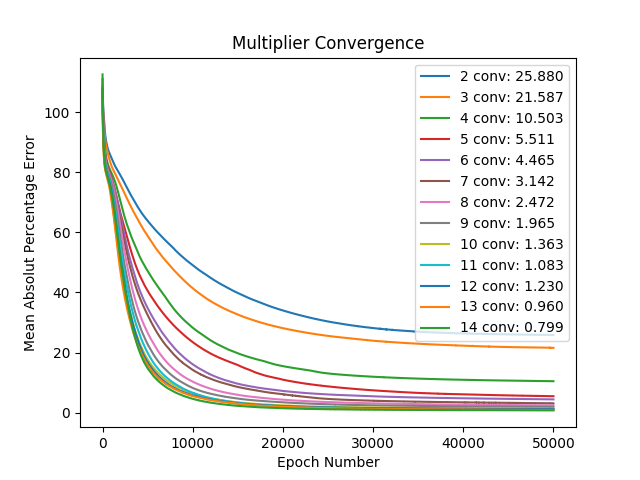
\includegraphics[scale=0.7]{learning/img/loss.png}
	\label{fig:mst_loss}
	\caption{Mit steigender Anzahl Neuronen im hidden Layer sinkt der relative Fehler gegen den im Training konvergiert wird.}
\end{figure}

\begin{figure}
	\centering
	\begin{tikzpicture}
	\node[inputNode, thick] (i1) at (6, 1) {};
	\node[inputNode, thick] (i2) at (6, 0) {};
	\node[inputNode, thick] (i3) at (6, -1) {};
	
	\node[inputNode, thick] (h_pre) at (8, 2) {};
	
	\node[inputNode, thick] (h1) at (10, 1) {};
	\node[inputNode, thick] (h2) at (10, 0) {};
	\node[inputNode, thick] (h3) at (10, -1) {};
	
	
	\node[inputNode, thick] (o1) at (12, 0.0) {};
	
	
	\draw[stateTransition] (5, 1) -- node[above] {$I_1$} (i1);
	\draw[stateTransition] (5, 0) -- node[above] {$I_2$} (i2);
	\draw[stateTransition] (5, -1) -- node[above] {$I_3$} (i3);
	
	
	
	\draw[stateTransition] (i1) -- (h1);
	\draw[stateTransition] (i1) -- (h2);
	\draw[stateTransition] (i1) -- (h3);
	\draw[stateTransition] (i1) -- (h_pre);
	
	\draw[stateTransition] (i2) -- (h1);
	\draw[stateTransition] (i2) -- (h2);
	\draw[stateTransition] (i2) -- (h3);
	\draw[stateTransition] (i2) -- (h_pre);
	
	
	\draw[stateTransition] (i3) -- (h1);
	\draw[stateTransition] (i3) -- (h2);
	\draw[stateTransition] (i3) -- (h3);
	\draw[stateTransition] (i3) -- (h_pre);
	
	\draw[stateTransition] (h_pre) -- (h1);
	\draw[stateTransition] (h_pre) -- (h2);
	\draw[stateTransition] (h_pre) -- (h3);
	
	
	\draw[stateTransition] (h1) -- (o1);
	\draw[stateTransition] (h2) -- (o1);
	\draw[stateTransition] (h3) -- (o1);
	
	\node[above=of i1, align=center] (l1) {Input \\ layer};
	\node[right=2.3em of l1, align=center] (l2) {Hidden \\ layer \#1};
	\node[right=2.3em of l2, align=center] (l3) {Hidden \\ layer \#2};
	
	\node[right=2.3em of l3, align=center] (l4) {Output \\ layer};
	
	
	\draw[stateTransition] (o1) -- node[above] {$O_1$} (13, 0);
	\end{tikzpicture}
	\label{fig:mst_variable_hidden_layer}
	\caption{Die vorgeschlagene Topologie des KNN zur Lösung der Burgersgleichung}
\end{figure}
